\chapter{Implementation}
\label{ch:implementation}

\section{Introduction}

This chapter describes the realized implementation of the Echora prototype, translating the requirements and system design presented in the previous chapters into a working software system. It documents the technology stack, the modular project structure, the sensing and perception subsystems, the feedback subsystems, and the datasets and model-training procedures used to build the custom perception models. All processing is performed locally on a PC, in line with the privacy-by-design and low-latency principles established earlier.

The implementation is organized as a single Python application that orchestrates an RGB-D sensing pipeline, a set of AI perception engines, a context-aware state machine, and multimodal (audio and haptic) feedback within a real-time frame-by-frame control loop.

\section{Development Environment and Technology Stack}

Echora is implemented in Python and executed within an isolated virtual environment. The system integrates several specialized computer-vision, deep-learning, and audio libraries, each responsible for a distinct part of the pipeline. Table~\ref{tab:tech_stack} summarizes the core technologies and their roles.

\begin{table}[H]
\centering
\begin{tabular}{|p{0.32\textwidth}|p{0.58\textwidth}|}
\hline
\textbf{Technology} & \textbf{Role in Echora} \\
\hline
DepthAI (OAK-D) & Synchronized RGB and stereo-depth acquisition, plus on-board IMU. \\
\hline
Ultralytics YOLOv8 & Obstacle detection, accessibility-control detection, and banknote detection, with built-in ByteTrack tracking. \\
\hline
PaddleOCR (PP-OCRv4) & Scene-text detection and recognition for the text-reading feature. \\
\hline
InsightFace (buffalo\_sc) & Face detection (RetinaFace) and 512-dimensional face embeddings (ArcFace). \\
\hline
MediaPipe Hands & Real-time hand and fingertip landmark tracking for hand guidance. \\
\hline
OpenCV & Image pre-processing, geometry, and the debugging visualization window. \\
\hline
pyttsx3 / Windows SAPI & Offline text-to-speech synthesis. \\
\hline
pygame & Low-latency playback of spatial audio alerts and tones. \\
\hline
SQLAlchemy / SQLite & Local persistence of face identities, preferences, and event logs. \\
\hline
Ollama (Gemma) & Optional vision-language model for background scene description. \\
\hline
PyTorch / Torchvision & Deep-learning runtime underpinning YOLOv8. \\
\hline
NumPy & Numerical processing of frames, depth maps, and embeddings. \\
\hline
\end{tabular}
\caption{Core technology stack of the Echora implementation}
\label{tab:tech_stack}
\end{table}

System configuration is centralized in a typed settings module based on \texttt{pydantic-settings}, allowing all thresholds, model paths, and timing parameters to be overridden through an \texttt{.env} file without modifying source code. Where a CUDA-capable GPU is available it is used automatically for inference; otherwise the system falls back to CPU execution.

\section{System Architecture and Project Structure}

The implementation follows a deeply modular architecture in which sensing and actuation are separated from perception and decision-making. The source code is organized into four packages:

\begin{itemize}
    \item \textbf{core} --- global configuration, shared utilities, the context-aware state machine, and the main control unit that drives the real-time loop.
    \item \textbf{perception} --- the AI engines: obstacle detection, the ByteTrack-based track lifecycle manager, OCR, face recognition, banknote detection, and interaction (hand-guidance) detection.
    \item \textbf{hardware} --- device interfaces: the depth camera, the audio-feedback engine, and the haptic-feedback engine.
    \item \textbf{storage} --- the local SQLite database and the face-registration workflow.
\end{itemize}

This separation allows each perception engine to be developed, tested, and replaced independently while the control unit coordinates them behind a stable interface. Figure~\ref{fig:impl_pipeline} shows how these packages cooperate at run time, from RGB-D acquisition through the perception engines to the decision and feedback stages.

\begin{figure}[H]
\centering
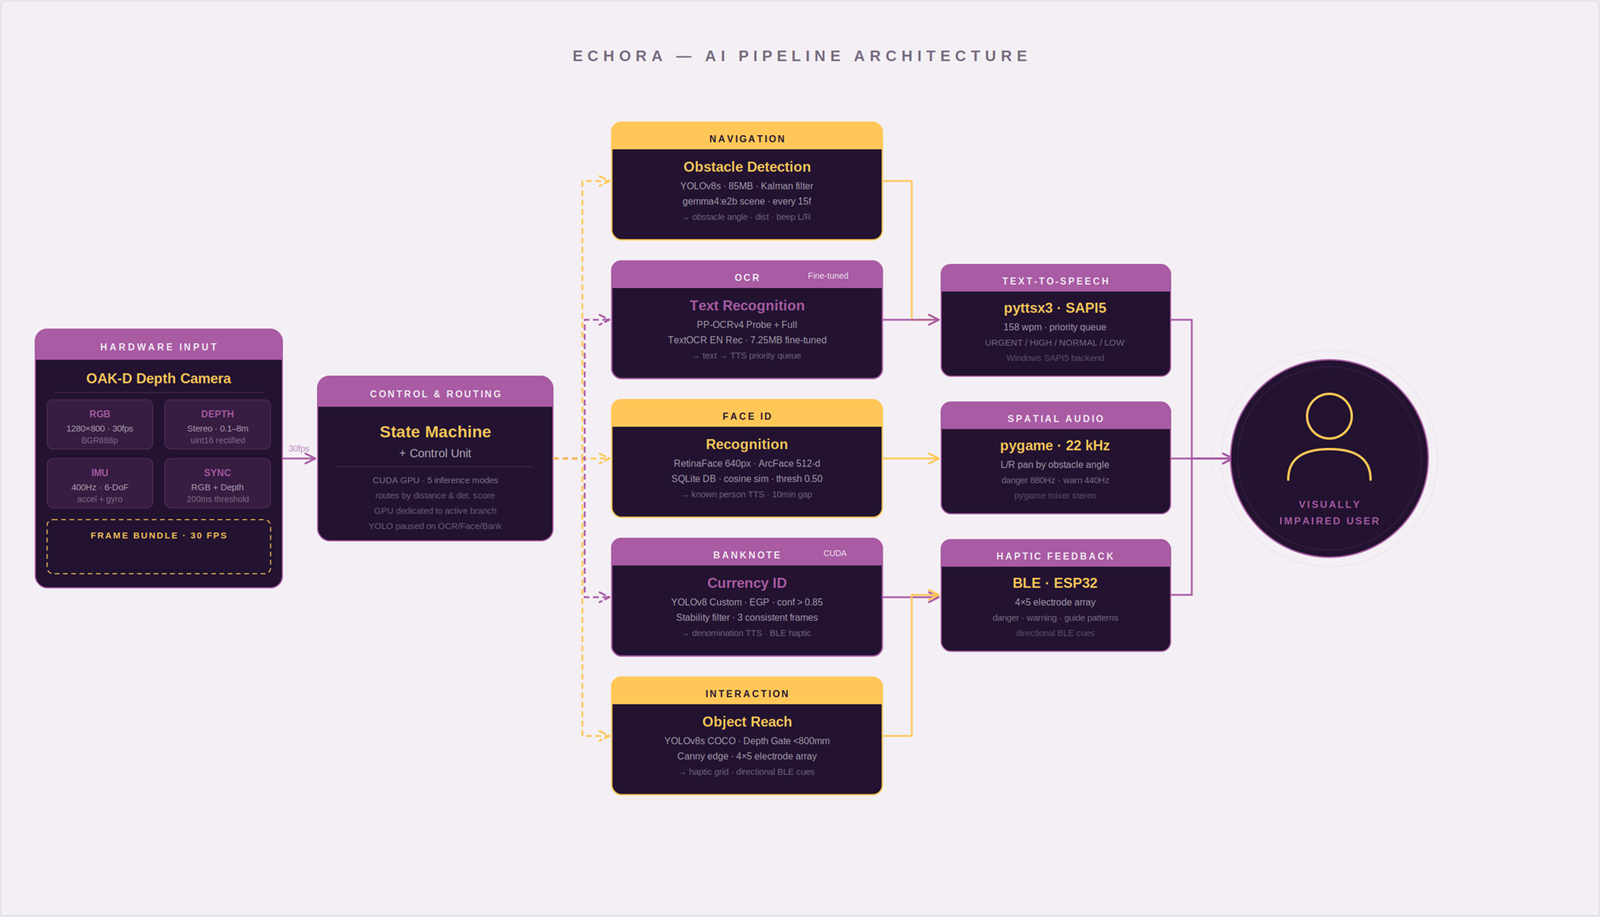
\includegraphics[width=\textwidth,height=0.85\textheight,keepaspectratio]{assets/implementation/ai_pipeline.png}
\caption{Echora AI pipeline architecture: from the OAK-D frame bundle, through mode routing in the control unit, to the per-mode perception engines and multimodal (audio and haptic) feedback delivered to the user.}
\label{fig:impl_pipeline}
\end{figure}

\section{Sensing and Data Acquisition}

The sensing layer is implemented around an OAK-D stereo camera using the DepthAI pipeline API. A single pipeline streams a color image from the central RGB sensor together with a stereo-depth map computed from the left and right mono sensors. The depth map is rectified and aligned to the RGB camera so that every detection can be associated with a per-pixel distance. Color and depth frames are paired using a synchronization node with a tolerance window, ensuring that perception always operates on temporally consistent RGB-D bundles.

The camera also exposes an on-board inertial measurement unit (IMU); accelerometer and gyroscope samples are collected on a dedicated thread and used by the state machine to estimate whether the user is stationary or in motion. Valid depth is constrained to a configured operating range, and a lightweight Kalman filter provides temporal smoothing of measurements, with tracks tolerated across a bounded number of consecutive missed frames before being discarded.

\section{Perception Subsystem}

\subsection{Obstacle Detection and Tracking}

Obstacle awareness is implemented in two cooperating layers. The first layer runs a YOLOv8 detector on every frame using Ultralytics' built-in tracking mode (ByteTrack), which associates detections across frames and recovers from short occlusions. Detections are restricted to a curated set of navigation-relevant classes (for example, people, furniture, doors, and stairs). Each detection's distance is sampled from the depth map within the inner region of its bounding box and mapped to a proximity zone: \emph{danger} within the configured danger distance, \emph{warning} within the warning distance, and \emph{safe} beyond it. Objects that fall inside the user's forward collision corridor are promoted to a higher urgency.

The second layer is a track-lifecycle manager layered on top of ByteTrack. Each track is modeled with an explicit state (\texttt{DETECTED}, \texttt{CONFIRMED}, or \texttt{LOST}); a track is promoted to \texttt{CONFIRMED} only after it is observed for a minimum number of consecutive frames, and it is deleted after a maximum number of consecutive missed frames. The manager maintains a short distance history per track and estimates the object's approach speed in millimeters per second (negative values indicate an object closing on the user), enabling the system to distinguish approaching hazards from receding ones. Only confirmed tracks are surfaced to the rest of the system. To enrich navigation without adding latency to the safety path, an optional vision-language model (Gemma, served locally through Ollama) runs asynchronously at a reduced rate to produce short natural-language scene descriptions; it is disabled automatically after repeated failures.

\subsection{Text Recognition (OCR)}

The text-reading feature is implemented with PaddleOCR's PP-OCRv4 detection and recognition models, augmented by a fine-tuned English recognition model (described in Section~\ref{sec:datasets}). Candidate frames are first checked for sharpness using a Laplacian-variance blur test, and a fast detection-only probe (cached for a short interval) decides whether text is present before the more expensive full recognition pass runs. Frames are pre-processed adaptively: contrast-limited adaptive histogram equalization (CLAHE) for dark scenes, gamma correction for over-bright scenes, bilateral denoising, and an unsharp-mask sharpening step.

Recognized words below a confidence threshold are discarded. To avoid speaking transient misreads, results are passed through a stability buffer that only accepts text appearing consistently across recent frames, and a repeat guard suppresses re-reading identical text within a cooldown period. The accepted text is then dispatched to the audio engine.

\subsection{Face Recognition}

Face recognition is implemented with the InsightFace \texttt{buffalo\_sc} model pack, which provides RetinaFace detection and ArcFace 512-dimensional embeddings via the ONNX runtime. Identity is determined by cosine similarity between the live embedding and stored embeddings, accepted only when the best match exceeds a recognition threshold and beats the runner-up by a configured margin, which reduces false identifications. A fast low-resolution detection probe runs periodically; full-resolution identification is triggered only when a face is present, and a stability buffer confirms an identity across several frames before it is announced. To avoid repetition, each recognized person is re-announced only after a configured absence interval.

\subsection{Banknote Recognition}

Currency recognition is implemented with a custom YOLOv8 detection model trained to localize and classify Egyptian Pound (EGP) denominations, including notes, coins, and the newer note designs (eleven classes in total). To ensure the user is actually holding a note, detections are only considered within a short distance from the camera, and a high confidence threshold is applied. A stability buffer requires agreement across consecutive frames before a denomination is announced, and a cooldown prevents the same note from being repeated within a short window.

\subsection{Interaction Detection and Hand Guidance}

Fine-grained interaction is implemented by combining MediaPipe Hands with the existing YOLO detections. MediaPipe provides 21 hand landmarks; the fingertip landmark is taken as the user's pointer, while the target object is selected from the YOLO detections restricted to interactable classes (such as handles and elevator controls). The system computes the three-dimensional offset between the fingertip and the target center --- horizontal and vertical displacement in pixels and depth difference in millimeters --- and drives a guidance state machine with phases \texttt{IDLE}, \texttt{GUIDANCE}, \texttt{EDGE}, and \texttt{SUCCESS} as the hand converges on the target.

The resulting direction (left, right, up, down, forward) and intensity are encoded onto a wrist-worn electro-tactile actuator grid, with intensity scaling as the hand approaches the target and a distinct confirmation pattern fired on success. The encoded commands are transmitted to the wearable wrist device over Bluetooth Low Energy.

\section{Datasets and Model Training}
\label{sec:datasets}

Three of Echora's perception models are custom-trained: the accessibility-control detector, the Egyptian banknote detector, and the fine-tuned English OCR recognizer. This section describes the datasets used and the training procedures.

\subsection{Accessibility Detection Dataset (Doors, Handles, and Elevator Controls)}

The accessibility detector is trained on a combined dataset built from two public Roboflow datasets: the \emph{Door and Handles Detection} dataset\footnote{\url{https://universe.roboflow.com/uaeu/door-and-handles-detection}} and the \emph{Elevator Button Recognition} dataset\footnote{\url{https://universe.roboflow.com/sun-moon-university/elevator-button-recognition}}. The door dataset contributes approximately 1,334 images across two classes (\texttt{door} and \texttt{door handle}), while the elevator dataset originally contains around 2,019 images annotated with a very large label space of button and indicator types.

A preparation script merges these sources into a focused seven-class dataset for interaction targets: \texttt{door}, \texttt{door handle}, \texttt{up}, \texttt{updown}, \texttt{close}, \texttt{down}, and \texttt{open}. All door images are retained, while elevator annotations are restricted to the five relevant control types and remapped accordingly; elevator frames that do not contain any of these controls are dropped. The resulting combined dataset contains \textbf{2,719 images} (2,156 for training, 289 for validation, and 274 for testing). Table~\ref{tab:accessibility_dataset} summarizes the composition.

\begin{table}[H]
\centering
\begin{tabular}{|l|c|c|c|c|}
\hline
\textbf{Source} & \textbf{Train} & \textbf{Validation} & \textbf{Test} & \textbf{Classes} \\
\hline
Door and Handles & 1,067 & 134 & 133 & door, door handle \\
\hline
Elevator (filtered) & 1,089 & 155 & 141 & up, updown, close, down, open \\
\hline
\textbf{Combined} & \textbf{2,156} & \textbf{289} & \textbf{274} & \textbf{7 classes} \\
\hline
\end{tabular}
\caption{Composition of the combined accessibility-detection dataset}
\label{tab:accessibility_dataset}
\end{table}

\begin{figure}[H]
\centering
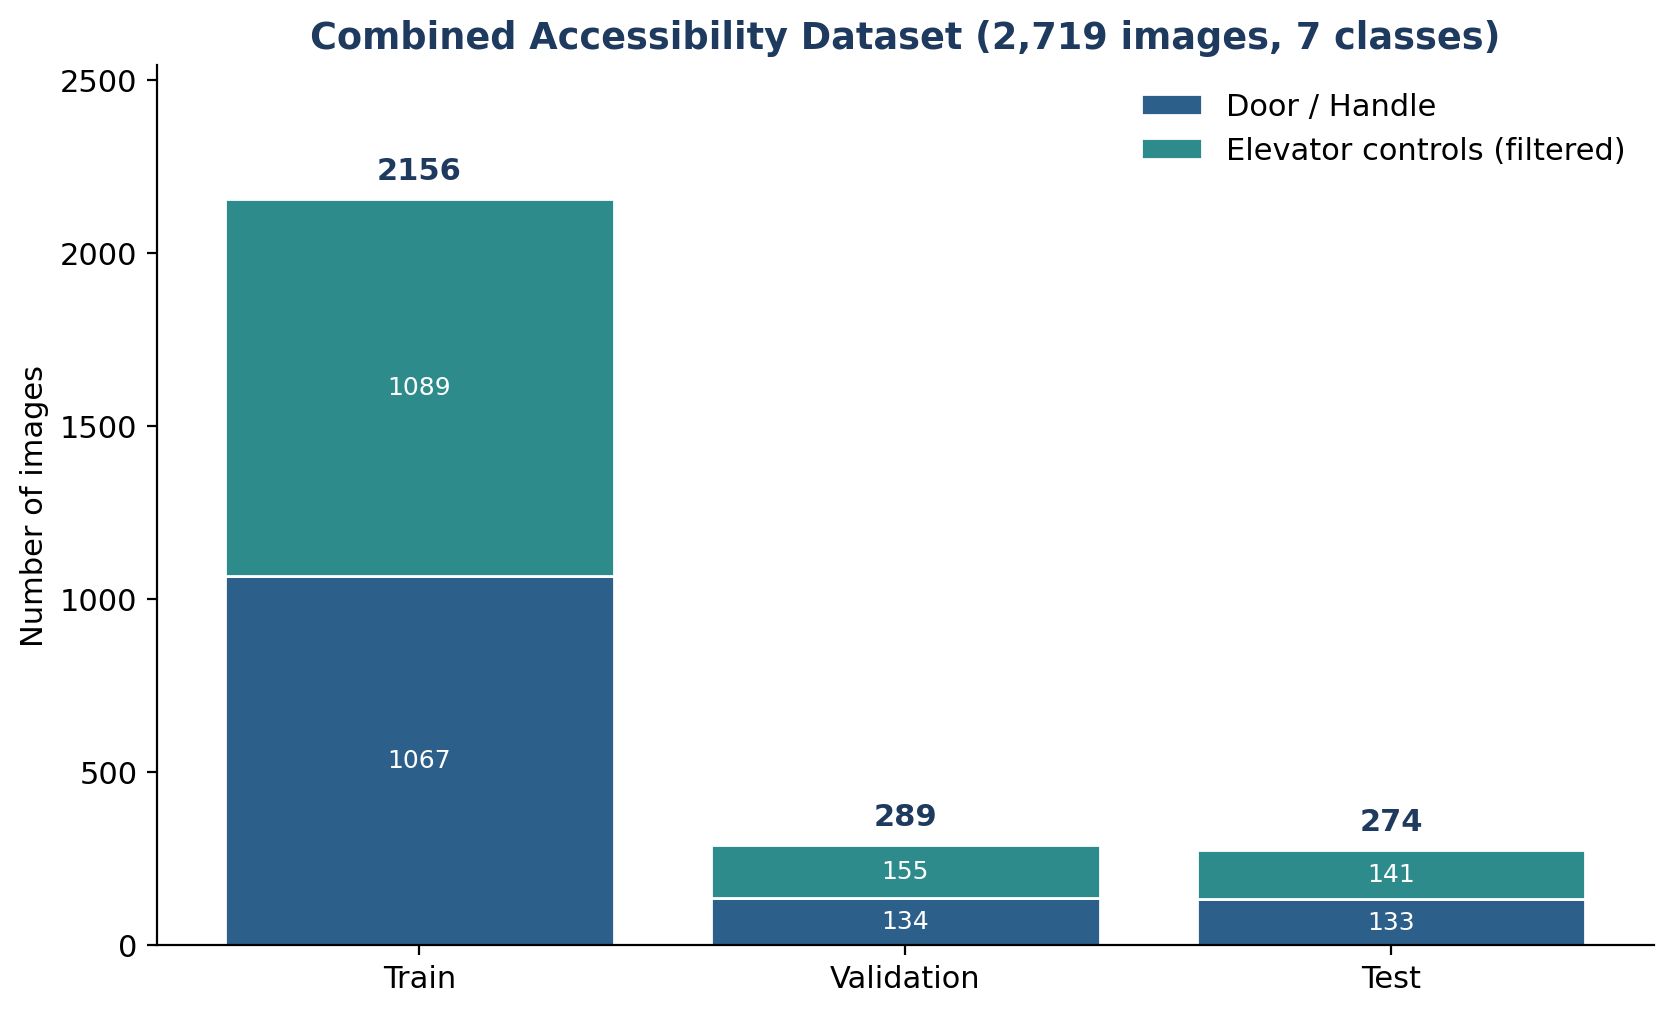
\includegraphics[width=0.85\textwidth,keepaspectratio]{assets/implementation/accessibility_dataset.png}
\caption{Combined accessibility-detection dataset composition across the train, validation, and test splits.}
\label{fig:accessibility_dataset}
\end{figure}

The model is a YOLOv8s detector fine-tuned from the pretrained \texttt{yolov8s} weights for 80 epochs at an input resolution of 640$\times$640, with a batch size of 8 and early-stopping patience of 20 epochs, on a CUDA GPU. The best checkpoint is exported as the runtime accessibility model.

\subsection{Egyptian Banknote Dataset (Custom)}

The banknote recognizer is trained on a custom dataset created by the authors specifically for this project\footnote{\url{https://app.roboflow.com/youssef-abdelrahman/egyptian_-banknote_yolov8/train}}, since no suitable public dataset of Egyptian currency was available. The dataset covers eleven denomination classes spanning notes, coins, and the newer note designs: \texttt{1\_EGP}, \texttt{1\_EGP\_coin}, \texttt{5\_EGP}, \texttt{10\_EGP}, \texttt{new\_10\_EGP}, \texttt{20\_EGP}, \texttt{new\_20\_EGP}, \texttt{50\_piastres}, \texttt{50\_EGP}, \texttt{100\_EGP}, and \texttt{200\_EGP}. Images were captured under varied lighting, backgrounds, and orientations to improve robustness, and were manually labeled by the Echora team as bounding boxes for a YOLOv8 detection model. The dataset comprises more than \textbf{7,400} annotated images, split 80\%/10\%/10\% into training, validation, and test subsets respectively (Figure~\ref{fig:banknote_dataset}). The detector is trained with YOLOv8 and deployed as the runtime banknote model.

\begin{figure}[H]
\centering
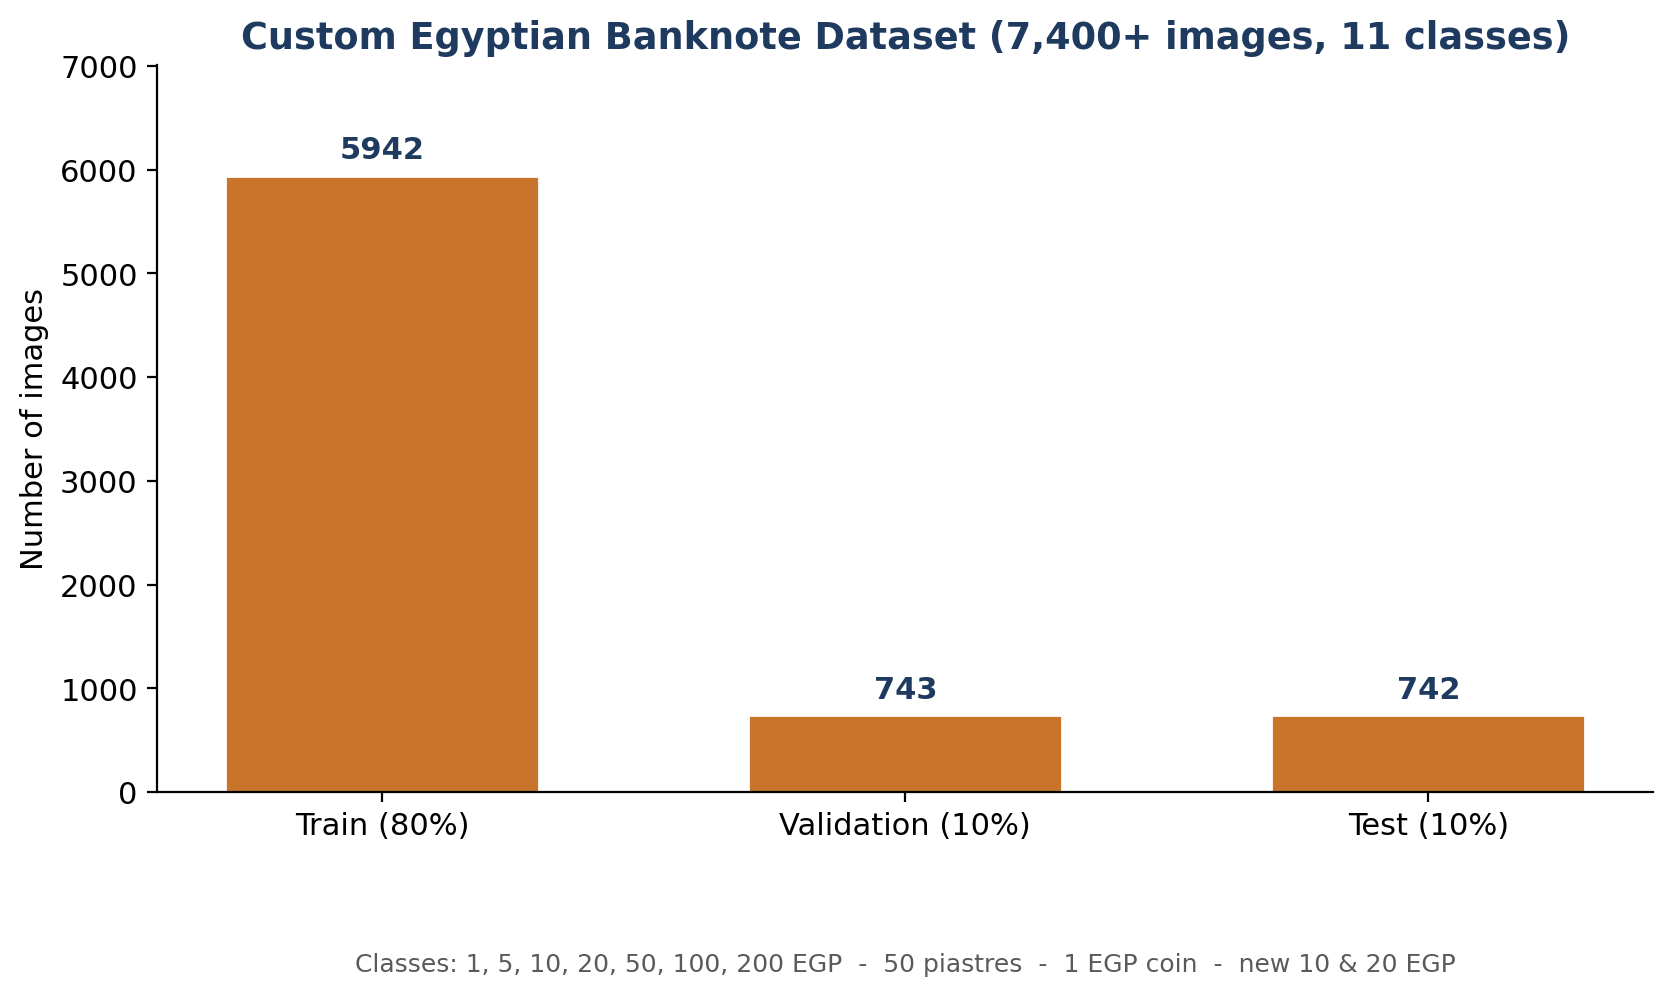
\includegraphics[width=0.85\textwidth,keepaspectratio]{assets/implementation/banknote_dataset.png}
\caption{Custom Egyptian banknote dataset: image counts across the train, validation, and test splits.}
\label{fig:banknote_dataset}
\end{figure}

\subsection{TextOCR Recognition Dataset}

To improve scene-text recognition over the default English model, the PP-OCRv4 recognizer is fine-tuned on the \emph{TextOCR --- Text Extraction from Images} dataset\footnote{\url{https://www.kaggle.com/datasets/robikscube/textocr-text-extraction-from-images-dataset}}. TextOCR is a large-scale scene-text dataset containing approximately 28,000 images with over 900,000 annotated words. A preparation script samples word-level annotations (by default around 12\% of the corpus), filters them to printable English words of reasonable length, crops each word region, and writes PaddleOCR-format \texttt{image}$\rightarrow$\texttt{text} label files, holding out a validation split.

The English PP-OCRv4 recognition model is then fine-tuned from the official pretrained weights for 15 epochs with a learning rate of $1\times10^{-4}$ and a batch size of 64 on a CUDA GPU. The exported inference model is loaded by the OCR engine at runtime, replacing the default English recognizer.

\section{Feedback Subsystem}

\subsection{Audio Feedback}

Audio is implemented as a priority-driven, non-blocking speech and alert system. Spoken messages are submitted to a priority queue (with urgency levels from urgent down to low) consumed by a dedicated worker thread, so that critical alerts can preempt routine announcements; a watchdog thread restarts the worker if it stalls. Speech synthesis uses pyttsx3, with a direct Windows SAPI fallback for robustness. Spatial alerts are rendered with pygame by panning a tone or sound effect between the left and right channels according to the object's bearing, giving the user an intuitive sense of direction, and per-alert cooldowns prevent the same cue from repeating too rapidly.

\subsection{Haptic Feedback}

Haptic feedback drives a wrist-worn actuator. Directional and proximity patterns --- and a dedicated success confirmation pattern --- are generated for the hand-guidance and danger workflows and transmitted to the wearable device over Bluetooth Low Energy. Pattern generation runs on background threads so that haptic output never blocks the perception loop.

\section{State Machine and Control Unit}

The behavior of Echora is coordinated by a context-aware state machine with five modes: \texttt{NAVIGATION} (the default), \texttt{OCR}, \texttt{INTERACTION}, \texttt{FACE\_ID}, and \texttt{BANKNOTE}. Transitions are driven by perception results combined with the IMU-derived motion estimate; for example, stable text within range while the user is nearly still triggers a switch to OCR, a nearby interactable object triggers INTERACTION, and a confidently detected face triggers FACE\_ID. To prevent unstable, rapid switching, each candidate transition must persist for a minimum number of frames, and each mode enforces a minimum dwell time before it can be exited. A detected danger-zone obstacle overrides all other modes and forces an immediate return to NAVIGATION, guaranteeing that safety alerts always take precedence. Figure~\ref{fig:impl_state_machine} summarizes the modes and their transitions.

\begin{figure}[H]
\centering
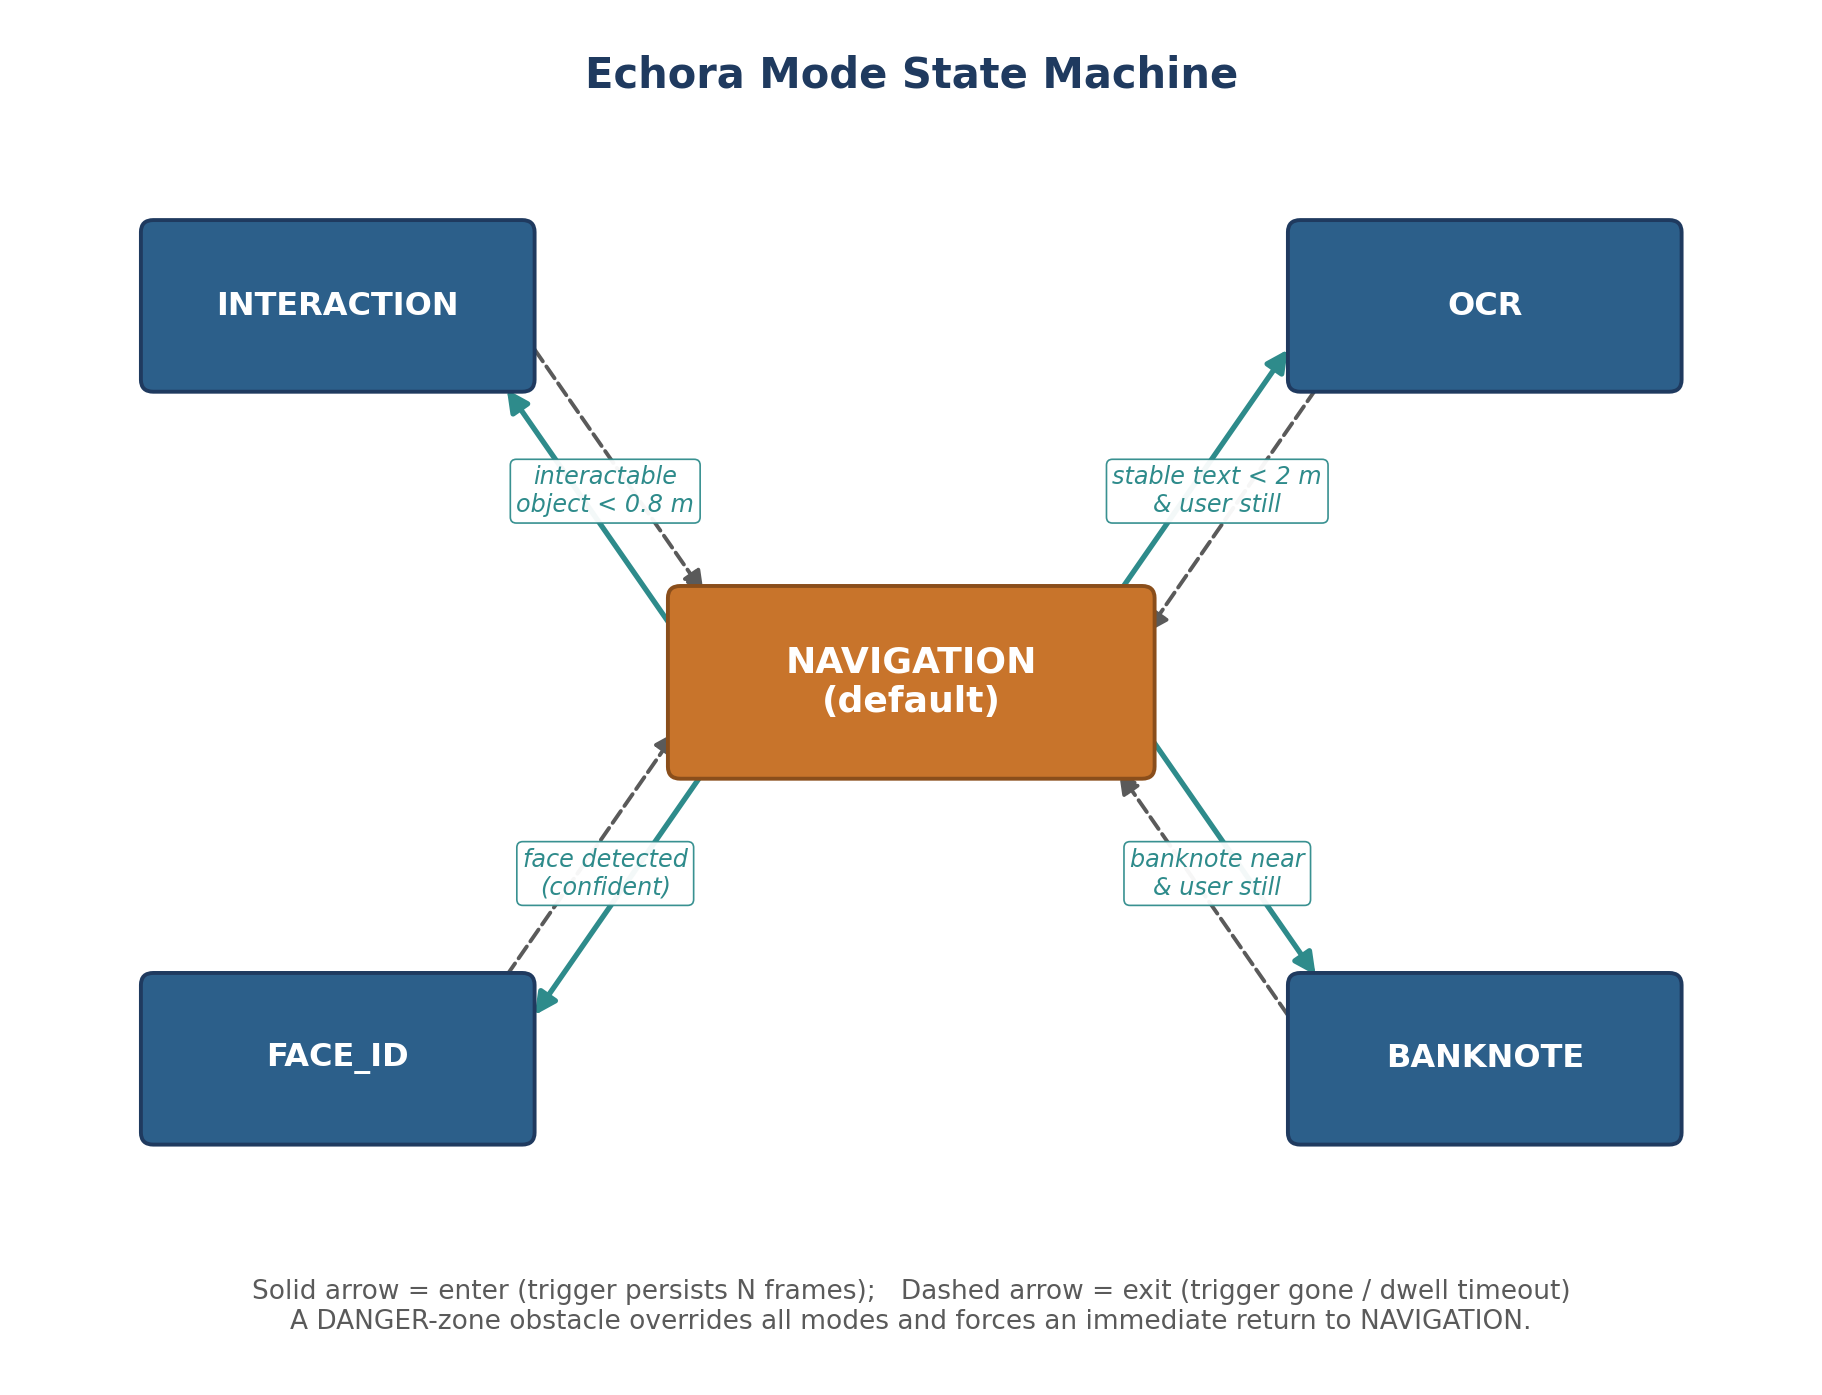
\includegraphics[width=\textwidth,height=0.6\textheight,keepaspectratio]{assets/implementation/state_machine.png}
\caption{Echora mode state machine: triggers (solid) and exits (dashed) around the default NAVIGATION mode.}
\label{fig:impl_state_machine}
\end{figure}

The control unit implements the real-time loop. On each iteration it retrieves a synchronized RGB-D bundle, runs obstacle detection every frame, runs the heavier engines (OCR probing, face detection, banknote detection, and interaction scanning) at reduced sub-frame intervals to balance computational load, evaluates the state machine, and dispatches the active mode's handler to produce audio and haptic output. Long-running operations such as OCR and face registration are executed on background threads to keep the loop responsive. The system supports both an automatic mode driven entirely by the state machine and a manual mode in which the operator selects modes by keyboard, and it logs per-frame timing to monitor real-time performance against the configured frame-time budget.

\section{Data Storage and Face Registration}

Persistence is implemented with SQLite through SQLAlchemy. The schema stores registered people (name, 512-dimensional embedding, first-seen and last-seen timestamps, and a sighting counter), user preferences, and an event log for recognitions and registrations. Embeddings are validated by size on load so that only compatible vectors are used.

Face registration is implemented as an interactive capture workflow: the operator enters a name, the system captures multiple frames over a short window, enforces quality gates (a minimum detection score and a minimum number of sharp frames), averages the best embeddings into a single normalized vector, and stores it against the provided name. Providing a name during this deliberate registration step constitutes the user's consent to store that identity.

\section{Evaluation and Testing}

This section reports the evaluation of the custom perception models and the testing of the application software. All detection metrics are produced by a reproducible harness (\texttt{scripts/evaluate\_models.py}) that runs each model against its held-out test split using the standard object-detection metrics: mean Average Precision at an IoU of 0.5 (mAP@0.5), mAP averaged over IoU thresholds 0.5--0.95 (mAP@0.5:0.95), precision, and recall.

\subsection{Accessibility Detection Model}

The accessibility detector was evaluated on its 274-image test split. Table~\ref{tab:acc_results} reports the overall and per-class results, and Figure~\ref{fig:cm_accessibility} shows the normalized confusion matrix.

\begin{table}[H]
\centering
\begin{tabular}{|l|c|c|c|c|}
\hline
\textbf{Class} & \textbf{Precision} & \textbf{Recall} & \textbf{mAP@0.5} & \textbf{mAP@0.5:0.95} \\
\hline
door & 0.866 & 0.874 & 0.913 & 0.741 \\
\hline
door handle & 0.787 & 0.758 & 0.793 & 0.444 \\
\hline
up & 0.812 & 0.755 & 0.774 & 0.623 \\
\hline
updown & 1.000 & 0.000 & 0.000 & 0.000 \\
\hline
close & 0.888 & 0.827 & 0.895 & 0.664 \\
\hline
down & 0.833 & 0.777 & 0.812 & 0.598 \\
\hline
open & 0.821 & 0.851 & 0.895 & 0.654 \\
\hline
\textbf{All classes} & \textbf{0.858} & \textbf{0.692} & \textbf{0.726} & \textbf{0.532} \\
\hline
\end{tabular}
\caption{Accessibility detection model results on the test split (YOLOv8s).}
\label{tab:acc_results}
\end{table}

\begin{figure}[H]
\centering

\includegraphics[width=0.78\textwidth,keepaspectratio]{assets/implementation/cm_accessibility.png}
\caption{Normalized confusion matrix for the accessibility detection model on the test split.}
\label{fig:cm_accessibility}
\end{figure}

The model achieves strong performance on the most safety- and interaction-relevant classes, with \texttt{door} (mAP@0.5 = 0.913), \texttt{close} (0.895), and \texttt{open} (0.895) leading. The \texttt{door handle} class is comparatively harder, reflecting its small object size. The \texttt{updown} class collapses to zero recall: it is severely under-represented in the test split, so the detector does not recover any of its few instances; expanding and balancing this class is a clear avenue for improvement. Overall, the detector reaches a mean precision of 0.858 and mAP@0.5 of 0.726, which is adequate for the assisted-interaction use case where detections are further stabilized by the ByteTrack lifecycle manager before being acted upon.

\subsection{Banknote Detection Model}

The Egyptian banknote detector was evaluated on its labeled held-out test set of 266 images, using the same harness and metrics as the accessibility model. Table~\ref{tab:banknote_results} reports the overall and per-denomination results, and Figure~\ref{fig:cm_banknote} shows the normalized confusion matrix.

\begin{table}[H]
\centering
\begin{tabular}{|l|c|c|c|c|}
\hline
\textbf{Class} & \textbf{Precision} & \textbf{Recall} & \textbf{mAP@0.5} & \textbf{mAP@0.5:0.95} \\
\hline
1 EGP & 0.994 & 1.000 & 0.995 & 0.981 \\
\hline
1 EGP (coin) & 1.000 & 1.000 & 0.995 & 0.986 \\
\hline
5 EGP & 0.997 & 1.000 & 0.995 & 0.982 \\
\hline
10 EGP & 0.994 & 1.000 & 0.995 & 0.989 \\
\hline
new 10 EGP & 1.000 & 1.000 & 0.995 & 0.982 \\
\hline
20 EGP & 1.000 & 1.000 & 0.995 & 0.975 \\
\hline
new 20 EGP & 1.000 & 1.000 & 0.995 & 0.974 \\
\hline
50 piastres & 0.996 & 1.000 & 0.995 & 0.990 \\
\hline
50 EGP & 0.996 & 1.000 & 0.995 & 0.984 \\
\hline
100 EGP & 0.995 & 1.000 & 0.995 & 0.995 \\
\hline
200 EGP & 0.997 & 0.960 & 0.955 & 0.936 \\
\hline
\textbf{All classes} & \textbf{0.997} & \textbf{0.996} & \textbf{0.991} & \textbf{0.979} \\
\hline
\end{tabular}
\caption{Banknote detection model results on the 266-image labeled test set (YOLOv8).}
\label{tab:banknote_results}
\end{table}

\begin{figure}[H]
\centering
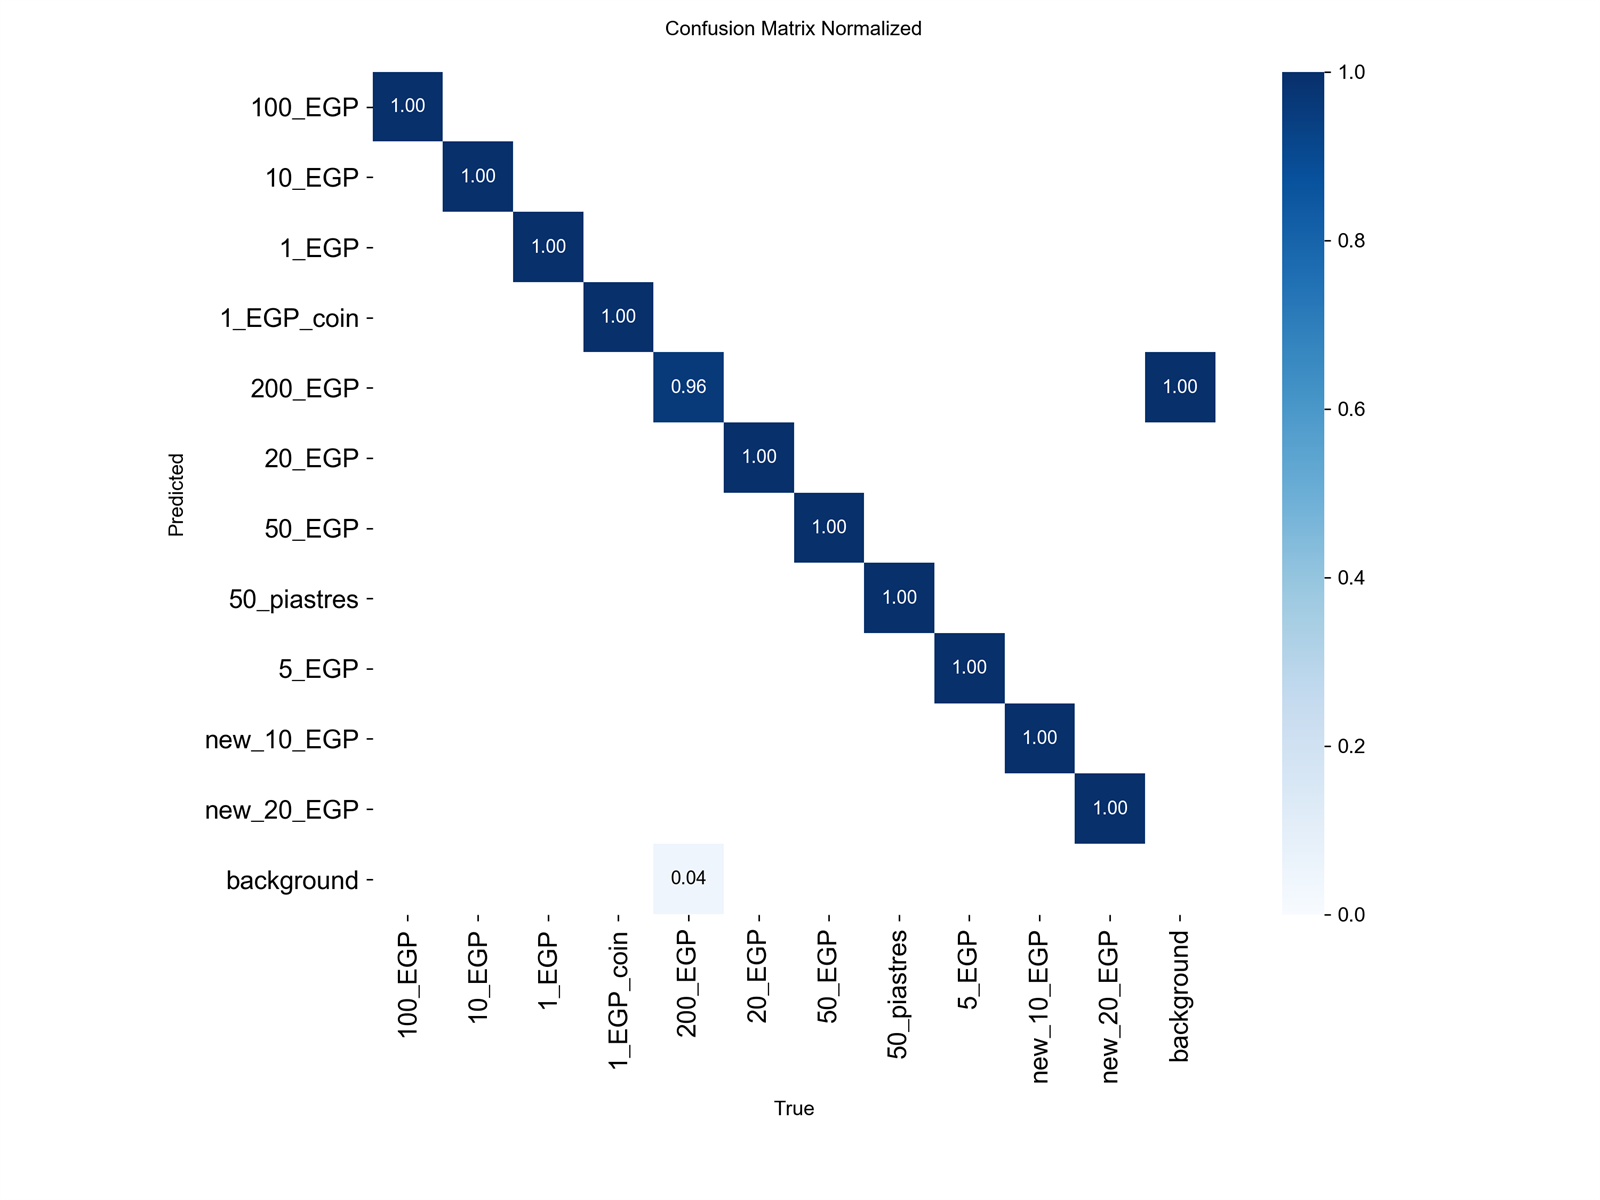
\includegraphics[width=0.78\textwidth,keepaspectratio]{assets/implementation/cm_banknote.png}
\caption{Normalized confusion matrix for the banknote detection model on the labeled test set.}
\label{fig:cm_banknote}
\end{figure}

The banknote detector achieves near-perfect performance, with an overall mAP@0.5 of 0.991, mAP@0.5:0.95 of 0.979, precision of 0.997, and recall of 0.996. Every denomination is recognized with an mAP@0.5 of at least 0.955, and the confusion matrix is almost purely diagonal. The only visible error is a small fraction of \texttt{200\_EGP} notes that go undetected (counted as background), which is reflected in that class's slightly lower recall of 0.960. These results confirm that the custom Egyptian banknote dataset and the trained detector are well-suited to the currency-identification task.

\subsection{Software Testing}

The application is accompanied by a test suite under \texttt{tests/} organized in two layers. The first layer consists of per-module self-test scripts (covering configuration, the state machine, utilities, and each perception and hardware engine) executed sequentially through \texttt{run\_tests.sh}. The second layer consists of automated integration (``runtime'') tests executed with \texttt{pytest}, which exercise the end-to-end behavior of the perception engines on sample inputs. As summarized in Table~\ref{tab:sw_tests}, all 22 automated integration tests pass.

\begin{table}[H]
\centering
\begin{tabular}{|l|c|c|}
\hline
\textbf{Test group} & \textbf{Cases} & \textbf{Result} \\
\hline
Obstacle detection (runtime) & 7 & Pass \\
\hline
OCR (runtime) & 8 & Pass \\
\hline
Interaction detection (runtime) & 4 & Pass \\
\hline
Banknote detection (runtime) & 2 & Pass \\
\hline
Audio feedback (runtime) & 1 & Pass \\
\hline
\textbf{Total} & \textbf{22} & \textbf{All pass} \\
\hline
\end{tabular}
\caption{Automated integration (pytest) test results.}
\label{tab:sw_tests}
\end{table}

\section{Summary}

This chapter presented the concrete implementation of Echora: the technology stack, the modular software architecture, the RGB-D sensing pipeline, the perception engines (obstacle detection with ByteTrack lifecycle management, OCR, face recognition, banknote detection, and hand-guidance interaction), the audio and haptic feedback subsystems, and the context-aware control loop. It also documented the three custom-trained models and the datasets behind them --- the combined accessibility-control dataset, the custom Egyptian banknote dataset, and the TextOCR fine-tuning corpus --- and reported the model evaluation (the accessibility detector reaching mAP@0.5 of 0.726 on its test split, and the banknote detector reaching mAP@0.5 of 0.991 on its labeled test set) together with the passing automated test suite. Together these components realize the design described in the previous chapters as a working, PC-local assistive prototype.
